\documentclass[11pt,a4paper]{scrartcl}
\usepackage[margin=1in,bottom=1.2in]{geometry}
\usepackage{amsfonts,amssymb,amsmath}
\usepackage[thmmarks,hyperref,amsthm,amsmath]{ntheorem} 
\usepackage{graphicx}
\usepackage[ruled,vlined,commentsnumbered]{algorithm2e}
\usepackage[usenames,dvipsnames]{color}
\usepackage{hyperref}
\usepackage{multirow}
\usepackage{lineno}
\usepackage[shortlabels]{enumitem}
\usepackage[utf8]{inputenc}
\usepackage[OT4]{fontenc}
\usepackage{comment}
\usepackage{fancyhdr}
\usepackage{tikz}

%Used Symbols
%c_i = chunk i
%v_i = vm i
%b_t = transfer bandwidth
%b_c = pairwise communication bandwidth
%n = |VMs| = |Chunks|


%Header Extensions Seperation
%Carlo
\newcommand{\VM}{\textsc{VM}}
\newcommand{\Chunk}{\textsc{chunk}}
\newcommand{\Problem}{\textsc{DummyName Problem}}

%Macieck

%Stefan

%End

\definecolor{blueLink}{rgb}{0,0.2,0.8}
\hypersetup{colorlinks,linkcolor=blueLink,urlcolor=blueLink,citecolor=blueLink}
\newcommand{\lref}[2][]{\hyperref[#2]{#1~\ref*{#2}}}



%%%%%%%%%%%%%%%%%%%%%%%%%%%%%%%%%%%%%%%%%%%%%%%%%%%%%%%%%%%%%
% GENERAL STYLE MACROS
%%%%%%%%%%%%%%%%%%%%%%%%%%%%%%%%%%%%%%%%%%%%%%%%%%%%%%%%%%%%%

\newcommand{\etal}{{\it et~al.\ }}
\newcommand{\myparagraph}[1]{{\smallskip\noindent{\bf #1}}}
\newcommand{\mycase}[1]{{\underline{Case~#1}:}}

%%%%%%%%%%%%%%%%%%%%%%%%%%%%%%%%%%%%%%%%%%%%%%%%%%%%%%%%%%%%
% THEOREMS AND SUCH
%%%%%%%%%%%%%%%%%%%%%%%%%%%%%%%%%%%%%%%%%%%%%%%%%%%%%%%%%%%%%

\newtheorem{theorem}{Theorem}
\newtheorem{corollary}[theorem]{Corollary}
\newtheorem{lemma}[theorem]{Lemma}
\newtheorem{claim}[theorem]{Claim}
\newtheorem{fact}{Fact}

%%%%%%%%%%%%%%%%%%%%%%%%%%%%%%%%%%%%%%%%%%%%%%%%%%%%%%%%%%%%%
% USEFUL LETTERS
%%%%%%%%%%%%%%%%%%%%%%%%%%%%%%%%%%%%%%%%%%%%%%%%%%%%%%%%%%%%%

\DeclareMathOperator{\polylog}{polylog}
\newcommand{\emdash}{\hspace{1mm}---\hspace{1mm}}
\newcommand{\e}{\mathrm{e}}
\renewcommand{\O}{\mathcal{O}}
\renewcommand{\Pr}{\mathbf{Pr}}
\newcommand{\E}{\mathbf{E}}
\newcommand{\NAT}{\mathbb{N}}
\newcommand{\REAL}{\mathbb{R}}

%%%%%%%%%%%%%%%%%%%%%%%%%%%%%%%%%%%%%%%%%%%%%%%%%%%%%%%%%%%%%
% PARENTHESES ETC
%%%%%%%%%%%%%%%%%%%%%%%%%%%%%%%%%%%%%%%%%%%%%%%%%%%%%%%%%%%%%

\newcommand{\ceiling}[1]{\left\lceil #1 \right\rceil}
\newcommand{\floor}[1]{\left\lfloor #1 \right\rfloor}
\newcommand{\braced}[1]{{\left\{#1\right\}}}
\newcommand{\bigbrackd}[1]{{\big[#1\big]}}
\newcommand{\brackd}[1]{{\left[#1\right]}}
\newcommand{\parend}[1]{{\left(#1\right)}}

%%%%%%%%%%%%%%%%%%%%%%%%%%%%%%%%%%%%%%%%%%%%%%%%%%%%%%%%%%%%%
% FRACTIONS
%%%%%%%%%%%%%%%%%%%%%%%%%%%%%%%%%%%%%%%%%%%%%%%%%%%%%%%%%%%%%

\newcommand{\half}{\frac{1}{2}}
\newcommand{\onehalf}{\frac{1}{2}}
\newcommand{\onethird}{\frac{1}{3}}
\newcommand{\twothirds}{{\textstyle\frac{2}{3}}}
\newcommand{\fourthirds}{{\textstyle\frac{4}{3}}}
\newcommand{\fivethirds}{{\textstyle\frac{5}{3}}}
\newcommand{\threefourths}{{\textstyle\frac{3}{4}}}

%%%%%%%%%%%%%%%%%%%%%%%%%%%%%%%%%%%%%%%%%%%%%%%%%%%%%%%%%%%%%
% ALGORITHM NAMES, ETC
%%%%%%%%%%%%%%%%%%%%%%%%%%%%%%%%%%%%%%%%%%%%%%%%%%%%%%%%%%%%%

\newcommand{\ALG}{\textsc{Alg}}
\newcommand{\OPT}{\textsc{Opt}}
\newcommand{\DET}{\textsc{Det}}
\newcommand{\RAND}{\textsc{Rand}}

%%%%%%%%%%%%%%%%%%%%%%%%%%%%%%%%%%%%%%%%%%%%%%%%%%%%%%%%%%%%%
% PSEUDOCODE
%%%%%%%%%%%%%%%%%%%%%%%%%%%%%%%%%%%%%%%%%%%%%%%%%%%%%%%%%%%%%

\newcommand{\IF}    {{\bf if }}
\newcommand{\THEN}  {{\bf then }} 
\newcommand{\FOR}   {{\bf for }}
\newcommand{\EACH}  {{\bf each }} 
\newcommand{\DO}  {{\bf do }} 

%%%%%%%%%%%%%%%%%%%%%%%%%%%%%%%%%%%%%%%%%%%%%%%%%%%%%%%%%%%%%
% EDITORIAL MACROS
%%%%%%%%%%%%%%%%%%%%%%%%%%%%%%%%%%%%%%%%%%%%%%%%%%%%%%%%%%%%%

\definecolor{brown}{rgb}{0.4,0,0} 
\definecolor{purple}{rgb}{0.2,0,0.6}
\definecolor{hotpink}{rgb}{1,0.4,0.7}
\newcommand{\marginnote}[1]{\marginpar{\scriptsize{\begin{flushleft}#1\end{flushleft}}}}
\newcommand{\todo}[1]{\noindent\colorbox{red}{todo: #1}} 
\newcommand{\marcin}[1]{\color{red} Marcin: #1\color{black}}



\title{Online Virtual Cluster Problem}
\author{List of authors here}

\begin{document}
\maketitle


\begin{abstract}
Abstract.
\end{abstract}

%%%%%%%%%%%%%%%%%%%%%%%%%%%%%%%%%%%%%
\section{Introduction}

%%%%%%%%%%%%%%%%%%%%%%%%%%%%%%%%%%%%%
\section{Preliminaries}


%%%%%%%%%%%%%%%%%%%%%%%%%%%%%%%%%%%%%
\section{Algorithms}

%%%%%%%%%%%%%%%%%%%%%%%%%%%%%%%%%%%%%%%
\subsection{Model variants}
\section{Model}

This section describes our model. We will start by describing a simplistic
version of our model, and continue to introduce new properties until we reach
the full model.

\subsection{Symbols}

This is a dummy section to introduce the symbols used later...

\begin{description}
 \item [$\Tree$] the substrate tree with $\Tree = (\SubstrateNodes , \SubstrateEdges)$
 \item [$\SubstrateNodes$]  a set of nodes: $\{\SubstrateNode_1, \dots ,
\SubstrateNode_{|\SubstrateNodes|}\}$
 \item [$\SubstrateEdges$] a set of edges : $\{\SubstrateEdge_1, \dots ,
 \SubstrateEdge_{|\SubstrateEdge|}\}$ with $\SubstrateEdge_1 =
(\SubstrateNode_i, \SubstrateNode_j)$
 \item [$c_i$] A chunk of type $i$
 \item [$v_i$] The i-th $\VM$ of the request
 \item [$\VirtualNodes$] the set of virtual Nodes = $\{1,2,\dots,\VCSwitch\}$
 \item [$\VirtualEdges$] the set of virtual Edges, $e_{V1}$ connects $1 \in
\VirtualNodes$ with $\VCSwitch \in \VirtualNodes$.
 \item [$\hat f$] the maximal flow
 \item [$|\hat f|$] the value of the maximal flow


 \item [$\Bandwidth$] Bandwidth constraint of an edge
 \item [$\CostTrans$] cost of chunk transport
 \item [$\CostCom$] cost of chunk communication
 \item [$\Vms$] number of VMs to spawn
 \item [$\ChunkTypes$] number of chunk types placed in an instance
 \item [$\Formula$] a formula
 \item [$\Clauses$] set of clauses in a formula
 \item [$\NClauses$] number of clauses in a given formula
 \item [$\Vars$] set of variables in a given formula
 \item [$\NVars$] number of variables in a given formula
 \item [$\Thr$] threshold
 \item [$\VCB$] virtual cluster model with bandwith
 \item [$\VCNB$] virtual cluster model without bandwith
 \item [$\varx$] variable
 \item [$\positive$] positive subtree of a gadget
 \item [$\negative$] negative subtree of a gadget
 \item [$\SAT$] set of satisfiable boolean formulas in CNF
 \item [$\TSAT$] set of satisfiable boolean formulas in 3CNF
 \item [$\Val$] valuation
 \item [$\Sol$] soultion to VC instance

\end{description}



\subsection{The Basic Model}

\carlo{Section TODO: How many / which figures + order?}

In the basic version of $\Problem$ data in the form of multiple chunks is
located in an undirected host graph tree $\Tree = (\SubstrateNodes,
\SubstrateEdges)$. A chunk $\Chunk$ of the set of chunks $\Chunks =
\{\Chunk_1,\dots,\Chunk_{\ChunkTypes}\}$ can only be located at the leaves
$\Leaves = \{\Leaf_1,\dots,\Leaf_m\} \subset \SubstrateNodes$ of $\Tree$. We
denote the location of a chunk by $\ChunkLocation : \Chunks \rightarrow
\Leaves$. A cluster, consisting of a set of VMs $\VirtualNodes =
\{\VirtualNode_1,\dots,\VirtualNode_{\Vms}\}$, is allready embedded on the host
graph, and should process this data. The VMs are embedded on the
leaves of the tree, and we denote the location of the VMs by $\NodeMapping :
\VirtualNodes \rightarrow \Leaves$. We assume that $\Vms = \ChunkTypes$, each
VM $\VirtualNode_i$ can read the data of one chunk $\Chunk_j$, and the data of
each chunk $\Chunk_j \in \Chunks$ has to be processed. In order to process the
data from a chunk $\Chunk_j$ with the VM $\VirtualNode_i$ it has to be
transferred along a (potentially empty) path $\Path_j =
\{\SubstrateEdge_{j_1},\dots,\SubstrateEdge_{j_n}\} ~ \SubstrateEdge_{j_k} \in
\SubstrateEdges$ such that $\SubstrateEdge_{j_1} = (\ChunkLocation(\Chunk_j),
\SubstrateNode_x)$, $\SubstrateEdge_{j_k} = (\SubstrateNode_x,
\SubstrateNode_y) \rightarrow \SubstrateEdge_{j_{k+1}} = (\SubstrateNode_y ,
\SubstrateNode_z)$, and $\SubstrateEdge_n = (\SubstrateNode_y,
\NodeMapping(\VirtualNode_i))$.  For the sake of simplicity we assume that
transferring a chunk over a link in the host graph inflicts bandwidth cost of
$\CostTrans$ on this link. The overall objective of $\Problem$ is to find an
assignment of VMs to chunks $\VmChunkAssignment : \Chunks \rightarrow
\SubstrateNodes$, so that the overall costs $\sum_{j \in
\{1,\dots,\ChunkTypes\}} |\Path_j|$ are minimized.

\begin{figure}

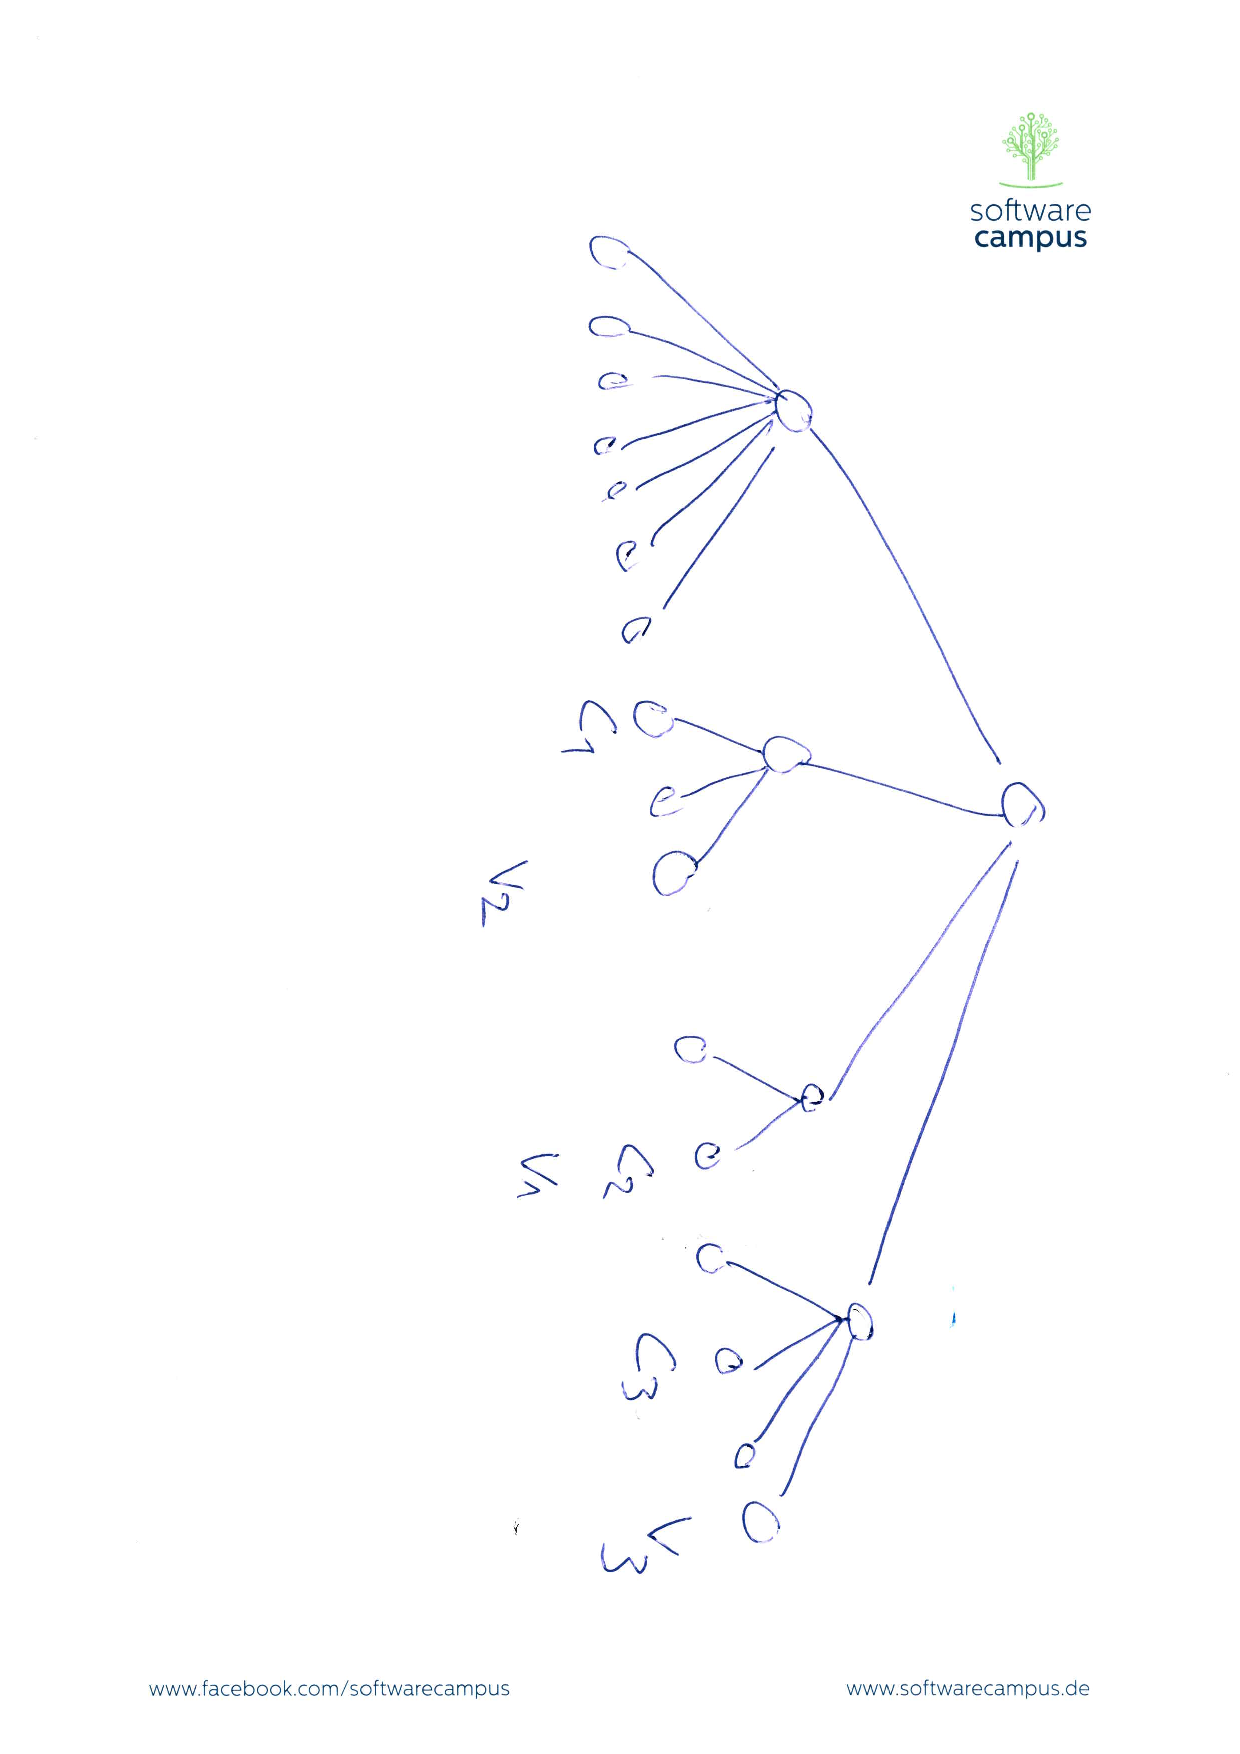
\includegraphics[angle=90,origin=c, height=7cm]{figs/model_fig_skteches/basic_problem}
\caption{basic problem}
\end{figure}
\begin{figure}

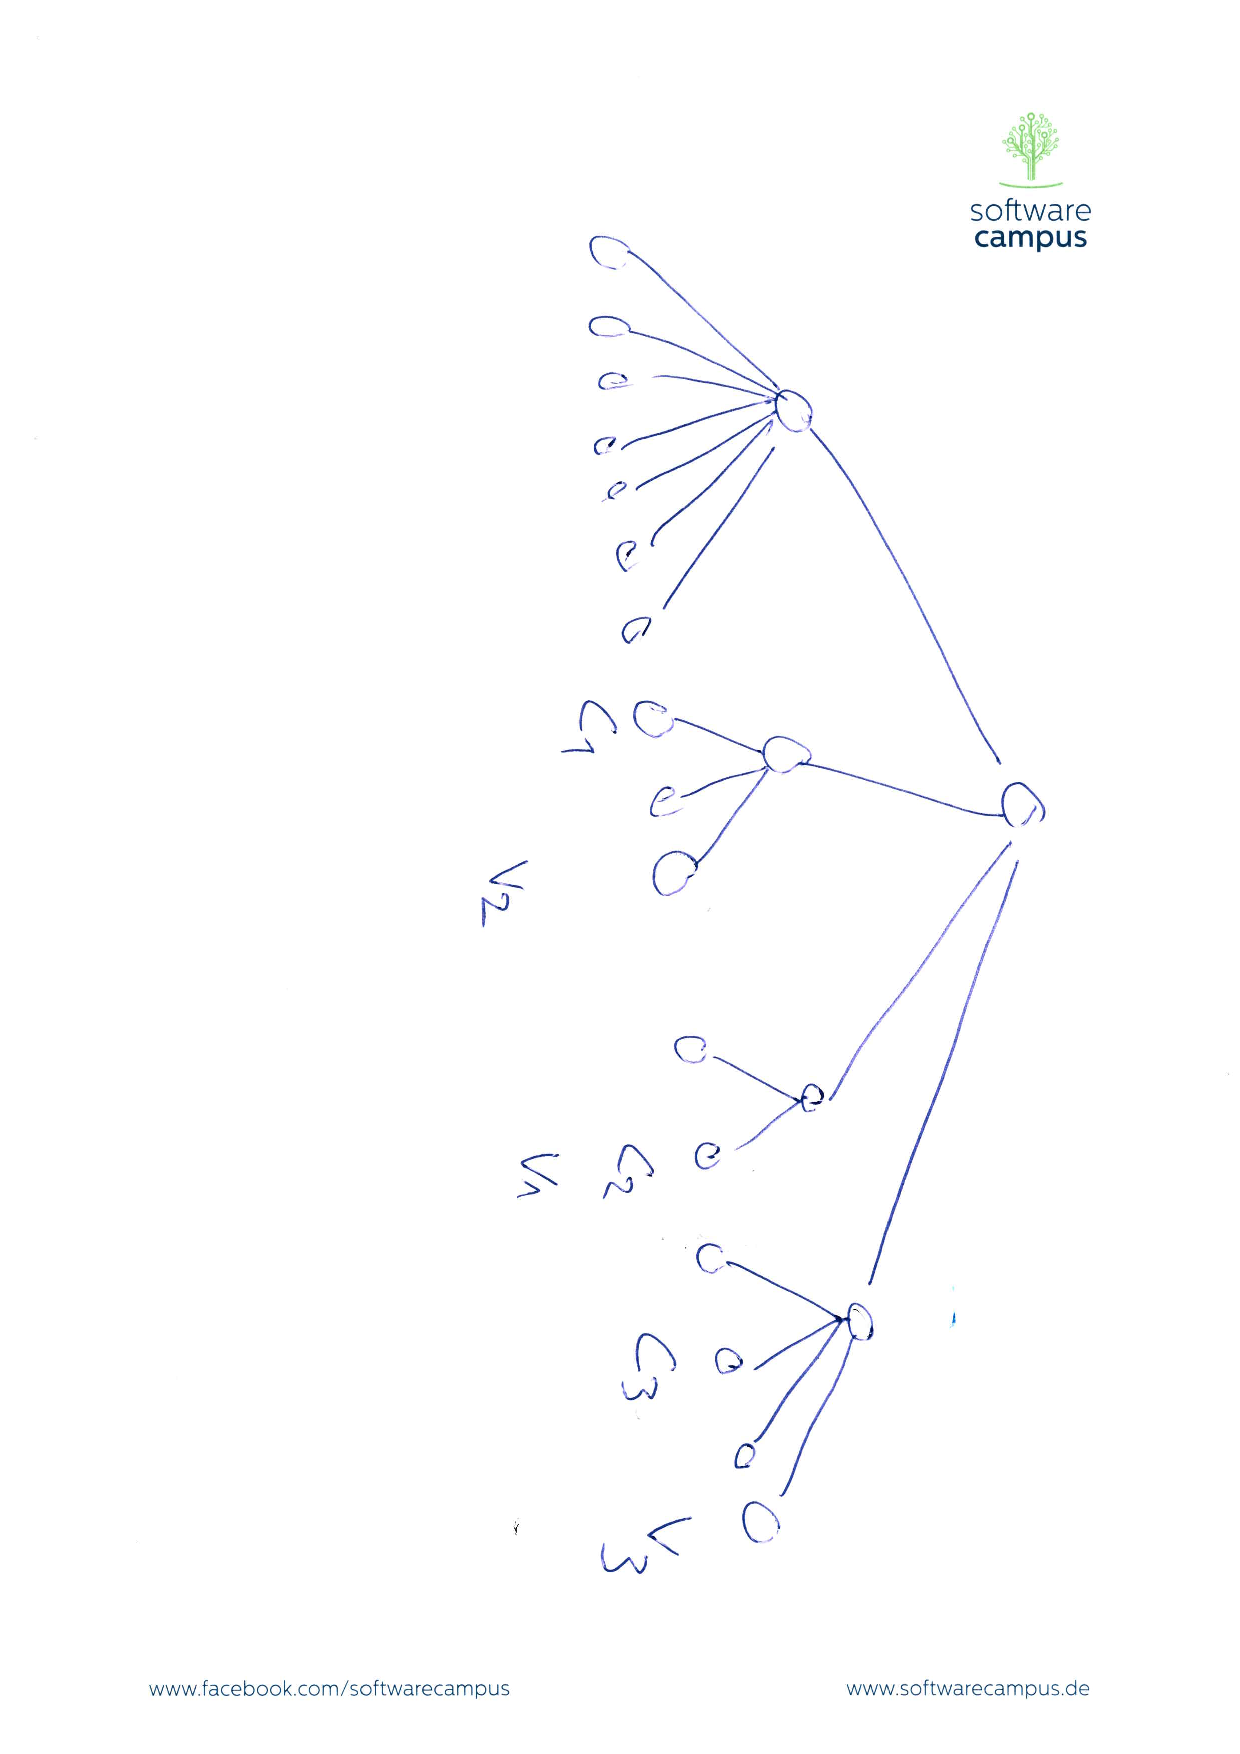
\includegraphics[angle=90,origin=c, height=7cm]{figs/model_fig_skteches/basic_problem}
\caption{solution for basic problem (green is pathes for transfer)}
\end{figure}

Throughout this section we will introduce different properties, to extend this
basic model. These properties can (and will) be combined to form more
challenging instances of $\Problem$.

%\begin{figure}[htbp]
%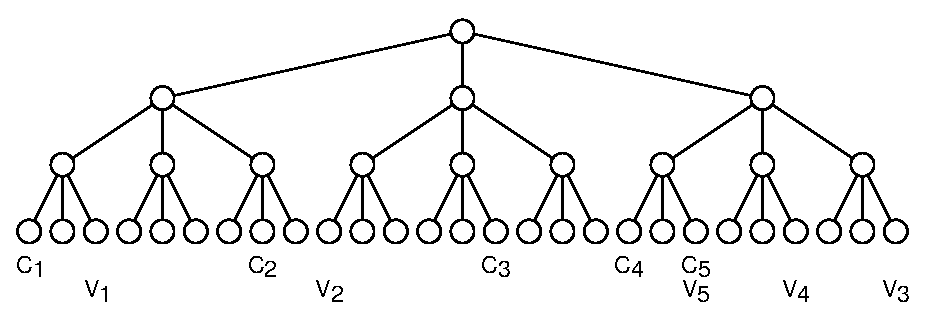
\includegraphics[width = \columnwidth]{figs/basic_scenario_3.eps}
%\caption{An example situation with 5 $\Chunk s$ and $\VM s$. Note that $c_5$
%and $v_5$ are on the same host.}
%\label{fig:model_clean}
%\end{figure}
%
%
%
%Figure~\ref{fig:model_clean} shows an example situation with $n = 5$. The goal
%of the $\Problem$  is to find an assignment of the $\VM s$ to the $\Chunk s$,
%which minimizes the overall bandwidth consumption of the job.
%
%We will now exemplarically examine an assignment of $\Chunk s$ to $\VM s$.
%Assume $c_1$ is assigned to $v_1$, $c2$ to $v2$, $c3$ to $v3$, $c4$ to $v4$
%and $c5$ to $v5$. Since $v_5$ runs on the same host, which contains $c_5$,
%transfering $c_5$ to $v_5$ will consume no bandwidth on the physical links.
%Hence we assume the overall bandwidth costs of the transfer to be $0$. The
%distrance between $v_1$ and $c_1$ is $2$ hops. Hence the transfer of the
%$\Chunk$ to the $\VM$ will consume bandwidth on two links. As a result, the
%overall bandwidth costs is $2 \cdot b_t$, where $b_t$ is the bandwidth
%neccessary for the transfer of a $\Chunk$. $v_4$ is $4$ hops away from $c_4$,
%which results in a total cost of $4 \cdot b_t$. Since the hop distance between
%$v_2$ and $c_2$ is 6, the costs for transferring the $\Chunk$ is $6 \cdot
%b_t$. The same holds for $v_3$ and $c_3$. The overall bandwidth consumption of
%the assignment is hence $18 \cdot b_t$.
%
%This is not an optimal solution for the $\Problem$. To show this, we will
%inspect a similar mapping. The only difference in the optimal mapping, is that
%$v_3$ is assigned to $c_2$ and $v_2$ is assigned to $c_3$. The bandwidth costs
%for transfering $c_2$ to it's assigned $\VM$ do not change, since $v_3$ is
%still $6$ hops away. $c_3$ however is now only $4$ hops away from its assigned
%$\VM$, which results in an overall bandwidth consumption of $16 \cdot b_t$.

\subsection{Communication Costs - $cv$}

\carlo{TODO: new symbol?}

This model extension assumes, that each VM  $\VirtualNode_i \in \VirtualNodes$
has to communicate with each other VM $\VirtualNode_{j \neq i} \in
\VirtualNodes$. Hence, the virtual cluster, which is to be embedded on the
physical substrate no longer consists only of a set of VMs, but is extended by a
set of virtual edges $\VirtualEdges : \VirtualNodes \times \VirtualNodes$.
Similar to the transfer of the chunks to the VMs, these edges have to be mapped
to a path in the host graph, which connects the locations to which the two VMs
are mapped. For the sake of simplicity we assume, that two VMs which communicate
inflict bandwidth cost of $\CostCom$ on each link of the path, which they use
for their communication.

\begin{figure}

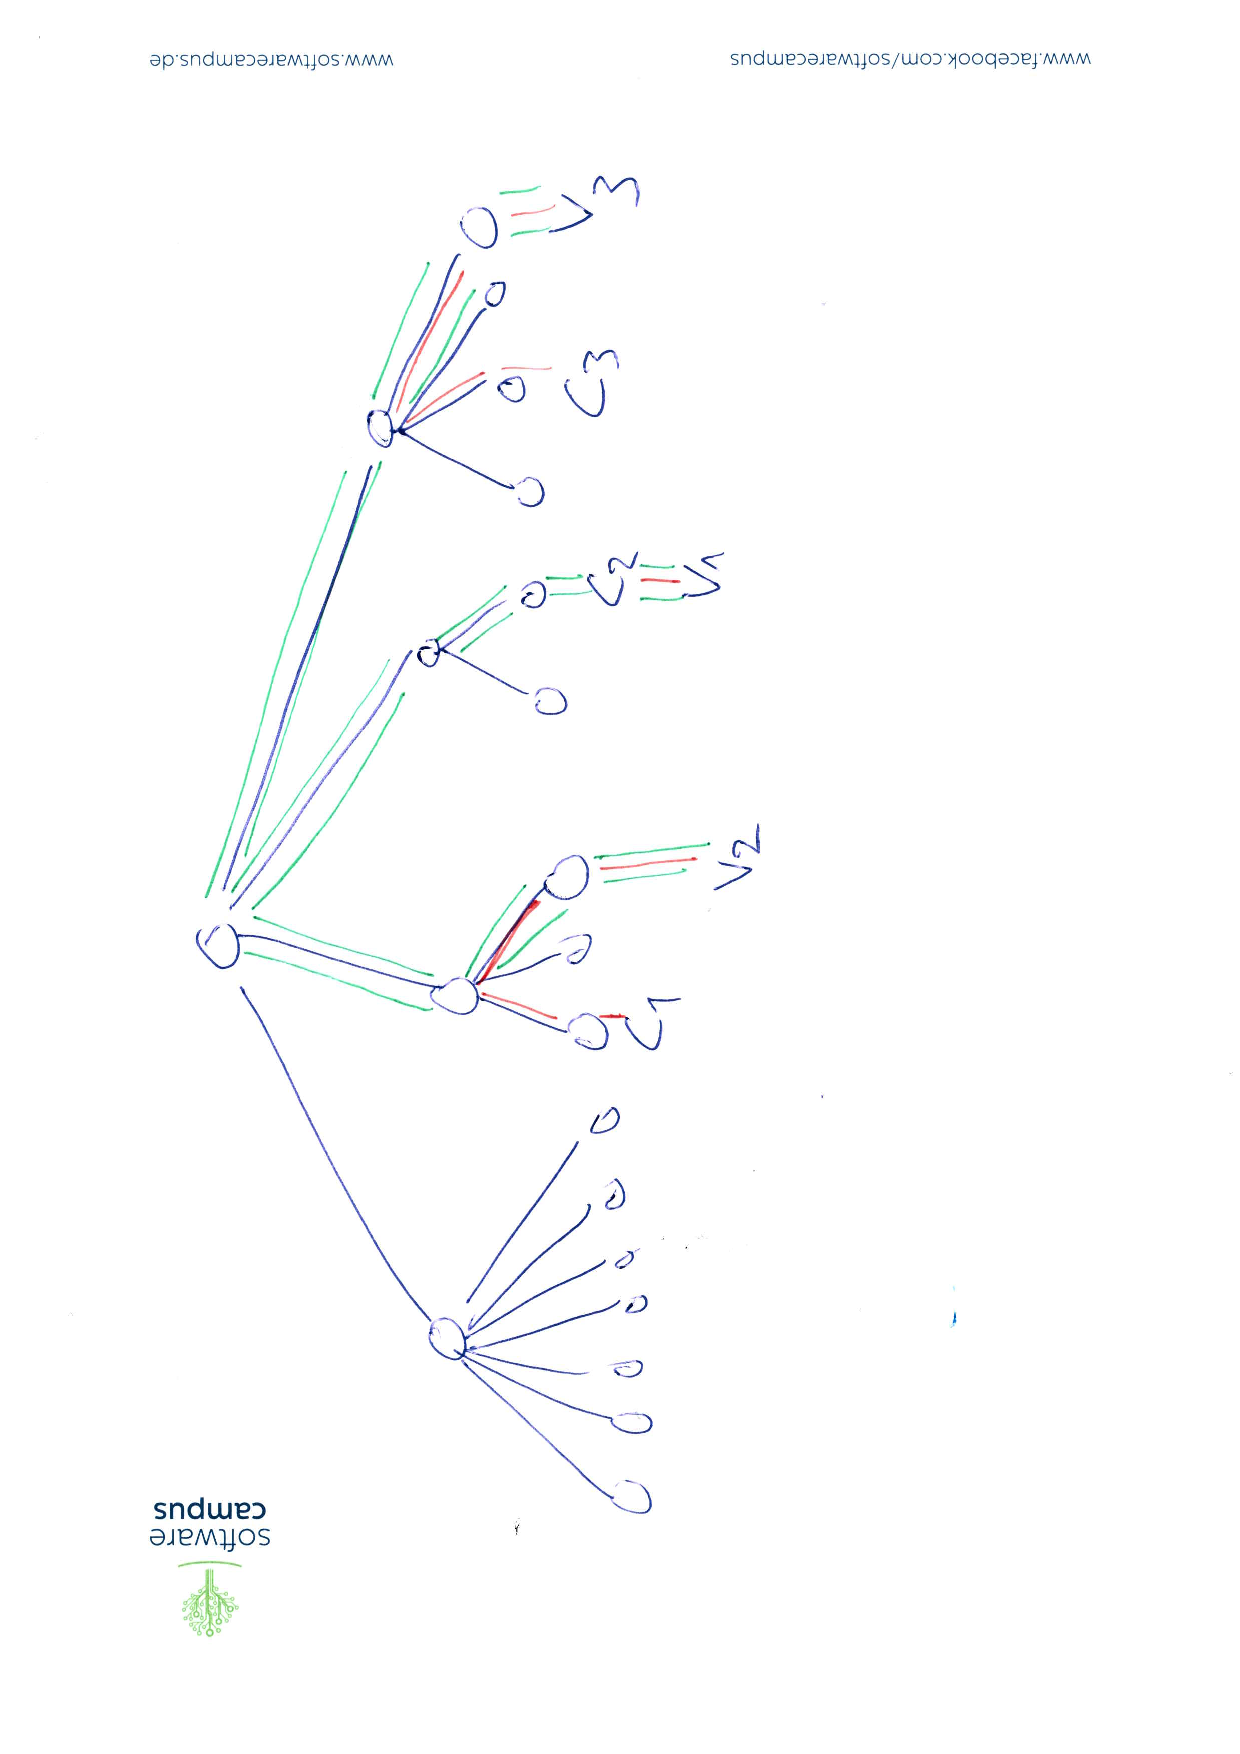
\includegraphics[angle=270,origin=c, height=7cm]{figs/model_fig_skteches/cv}
\caption{solution for problem with cv}
\end{figure}

%So
%far our model accounted bandwidth which is consumed to transfer data from it's
%location in the physical topology to the $\VM$ which will process it. However,
%due to the nature of distributed jobs, the $\VM s$ will also comunicate with
%each other. While we denoted the costs of transfering a chunk over a (1-hop)
%link with $b_t$, we will refer to the bandwidth costs of transfering data
%between a pair of $\VM s$ with $b_c$.


\subsection{Redundant Chunks - $r$}

This property specifies that, instead of having a single chunk $\Chunk_j$, we
have $\RedundancyFactor$ redundant copies of each chunk
$\Chunk_{j_1},\dots,\Chunk_{j_\RedundancyFactor}  \in \Chunks$. These copies are
entirely equal, and only one instance of a specific chunk type (e.g.
$\Chunk_{j_2}$) has to be read by one VM $\VirtualNode_j \in \VirtualNodes$.
Note that we assume chunks to be atomic - they cannot be read from two different
locations, requiering only $\CostTrans / 2$  bandwidth.

\begin{figure}

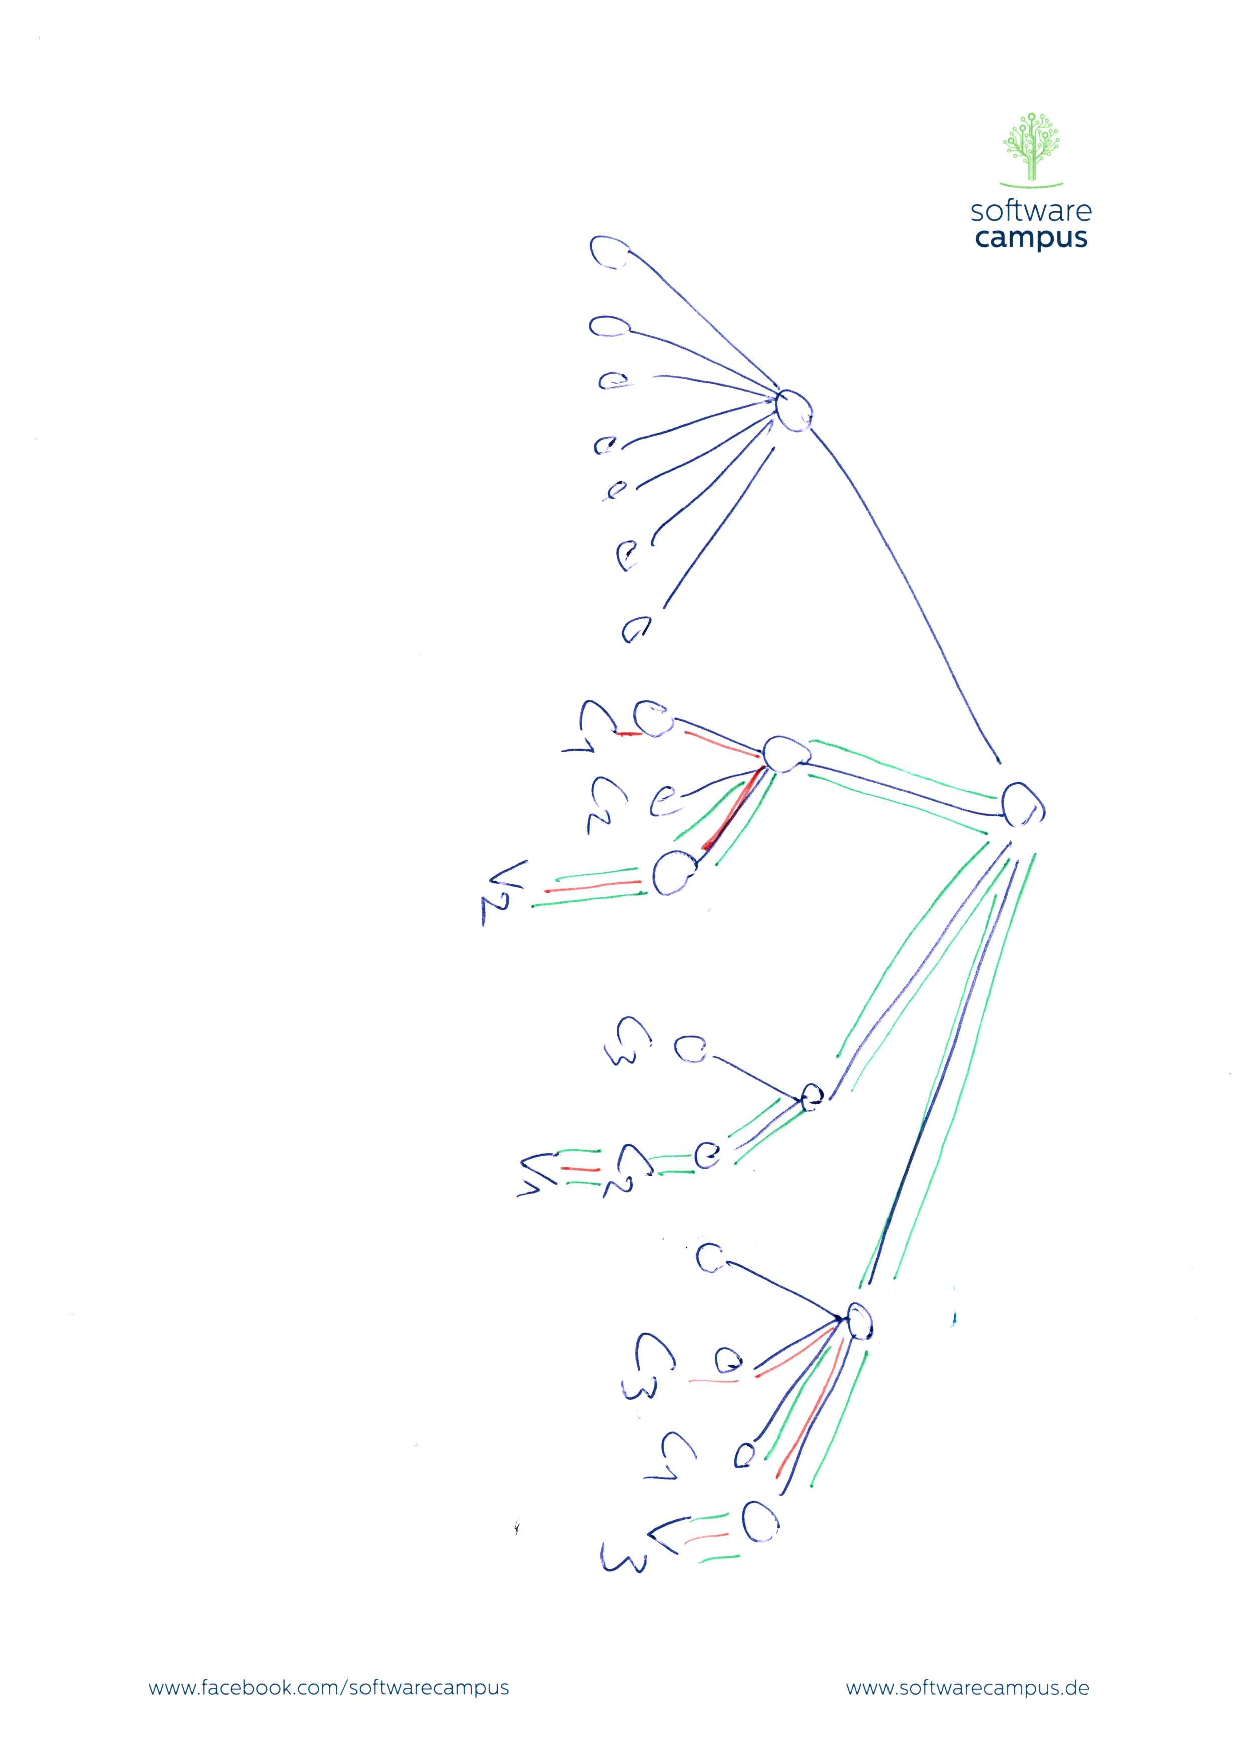
\includegraphics[angle=90,origin=c, height=7cm]{figs/model_fig_skteches/r_cv}
\caption{solution for problem with r}
\end{figure}




\subsection{Multiple Chunks per VM - $ma$}

This extension increases the processing capacities of the VMs. Instead of the
basic 1:1 ratio of VMs and chunks, this extension allows a VM to process
$\MaFactor \in \mathbb{N}^+$ many chunks. We assume, that the data which has to
be transferred to the VM from the chunks cannot be aggregated, and $\Vms =
\ChunkTypes / \MaFactor$.

\begin{figure}

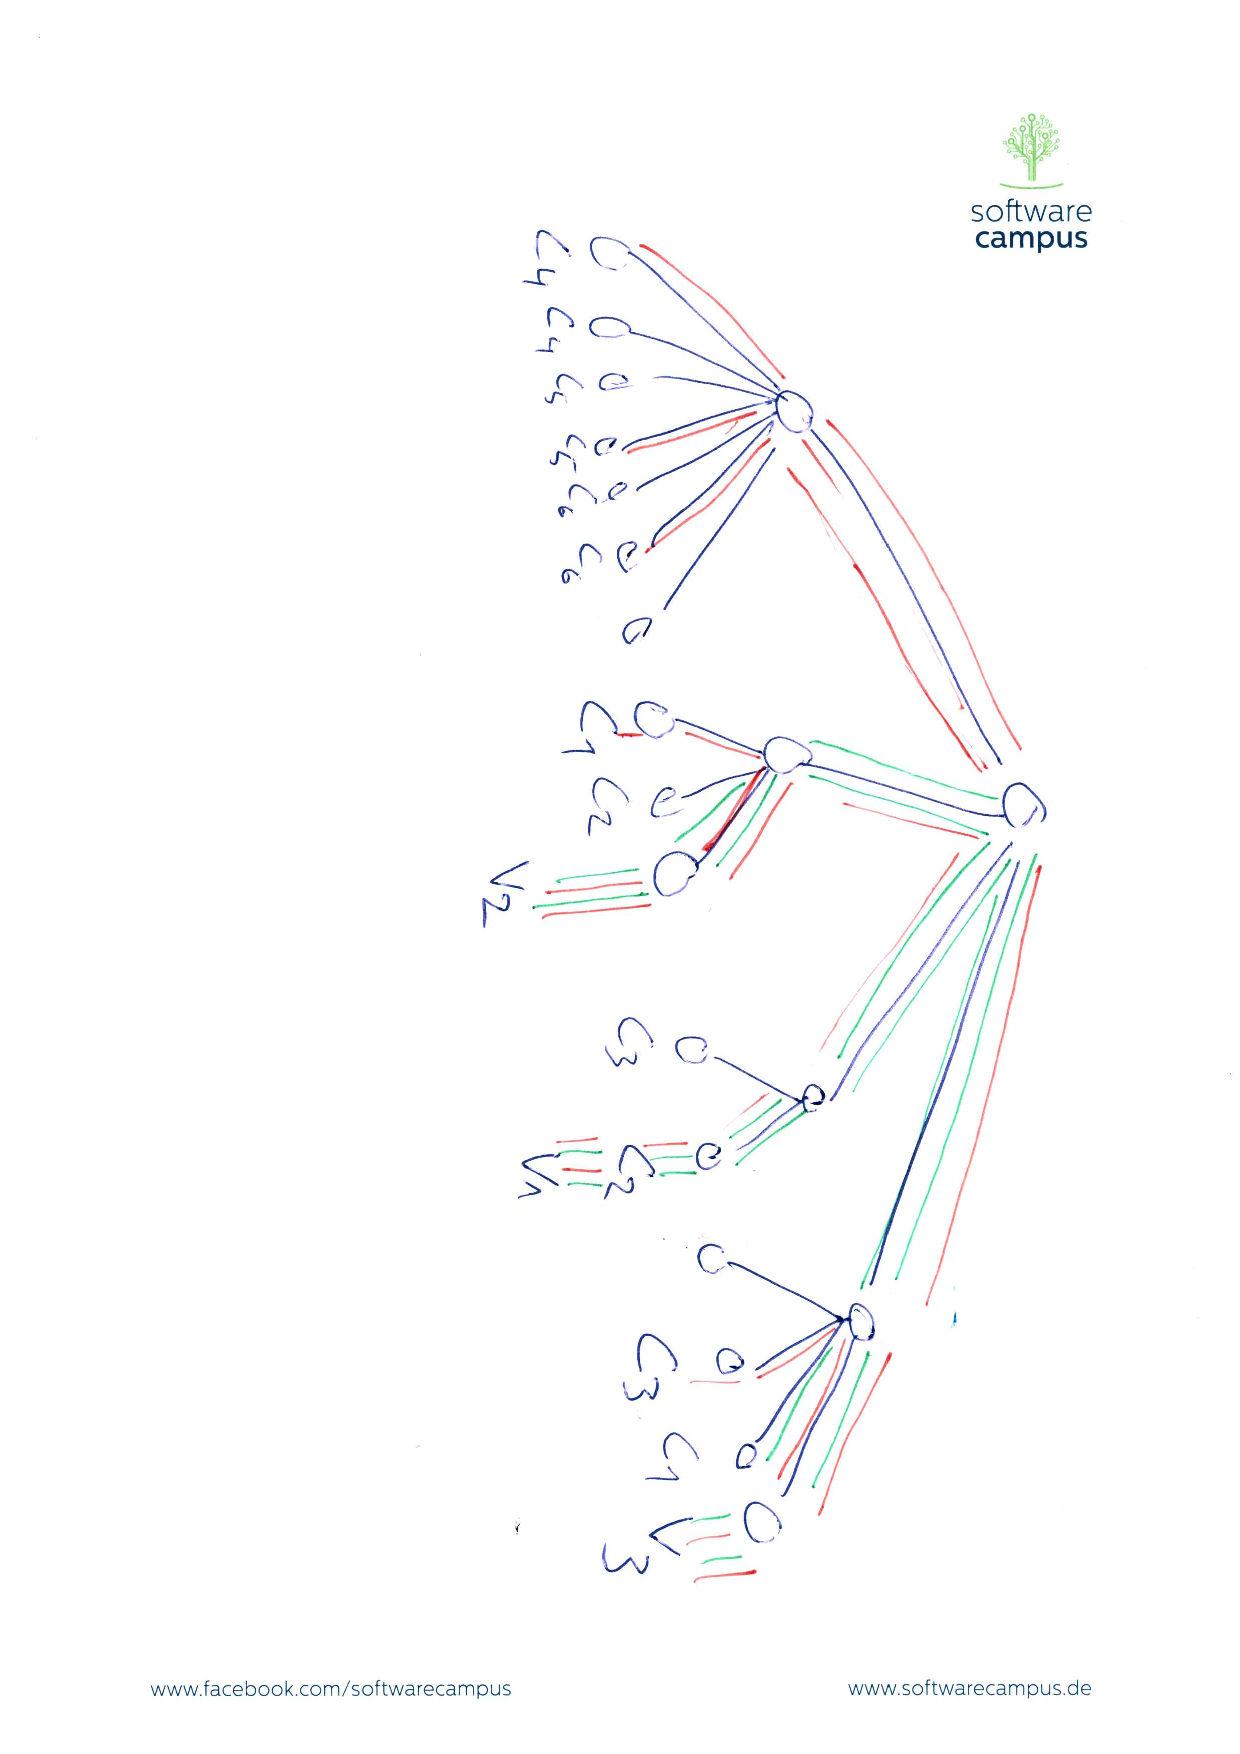
\includegraphics[angle=90,origin=c, height=7cm]{figs/model_fig_skteches/ma_r_cv}
\caption{soltion with ma}
\end{figure}

\subsection{Bandwidth Constraints - $bw$}

So far we only focussed on computing minimal bandwidth costs. However, in
reality the bandwidth which a single link can offer is limited. This model
extension limits the available bandwidth on each link $\SubstrateEdge_i \in
\SubstrateEdges$ in the host graph $\Tree$. We denote the capacity limitations
by $\Capacity : \SubstrateEdges \rightarrow \mathbb{R}$. The sum of all
bandwidth costs on this link, may never exeed it's capacity. Be aware that
this extension introduces infeasible instances.

\begin{figure}

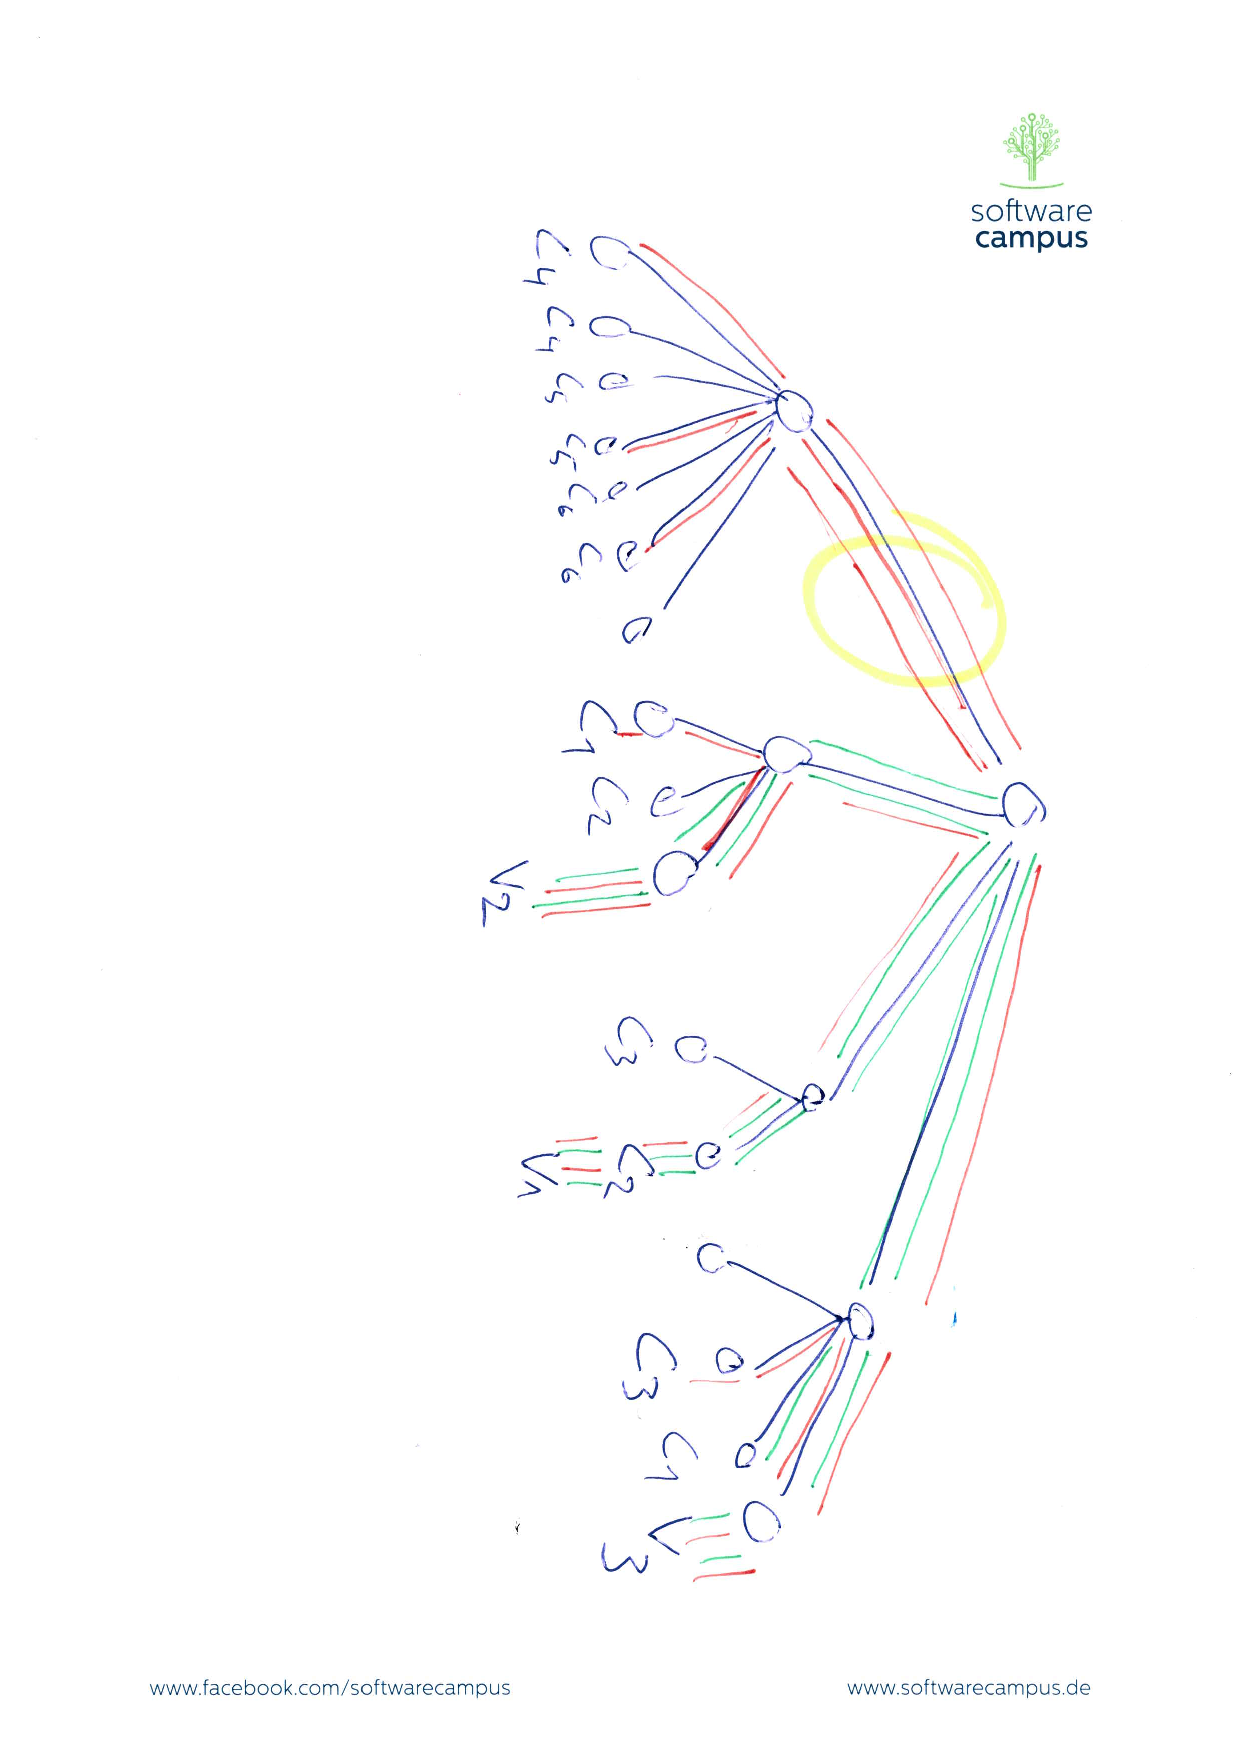
\includegraphics[angle=90,origin=c, height=7cm]{figs/model_fig_skteches/bw_ma_r_cv}
\caption{The bandwidth exceeds the capacity - independent of the chosen assignment}
\end{figure}
\subsection{Free VM Placement - $fp$}

The Free VM Placement property describes a variant of our simple model, where
the positions of the VMs are not given in the problem statement but are
rather chosen by the described strategy. Concretely, $\NodeMapping$ is no
longer given, but part of the optimization within $\Problem$. We assume that
each leaf can only host one VM.


\subsection{Summary of our results}

One day there will be a graph of all problems with arrows
corresponding to reductions and with partitioning to solution
approaches ((M)atching, (D)ynamic, (F)low, (N)p-hard).

\begin{enumerate}
\item basic problem - M
\item ma - M
\item r - M
\item cv - reduces to basic problem
\item bw - F
\item fp - solution of 0 cost
\item ma + r - M
\item  ma + bw - F
\item ma + cv - reduces to ma
\item ma + fp - D
\item r + bw - F
\item r + cv - reduces to r
\item r + fp - solution of 0 cost
\item bw + cv - reduces to bw
\item bw + fp - D
\item fp + cv - D
\item ma + r + bw - F
\item ma + r + cv - reduces to ma + r
\item ma + r + fp - N
\item ma + bw + cv - reduces to ma + bw
\item ma + bw + fp - D
\item ma + fp + cv - D
\item r + bw + cv - reduces to r + bw
\item r + cv + fp - N
\item r + bw + fp - solution of 0 cost
\item bw + cv + fp - D
\item ma + r + bw + cv - reduces to ma + r + bw
\item ma + r + bw + fp - N
\item ma + r + cv + fp - N
\item ma + fp + cv + bw - D
\item r + bw + cv + fp - N
\item ma + r + bw + cv + fp - N
\end{enumerate}


\begin{figure}[htbp]
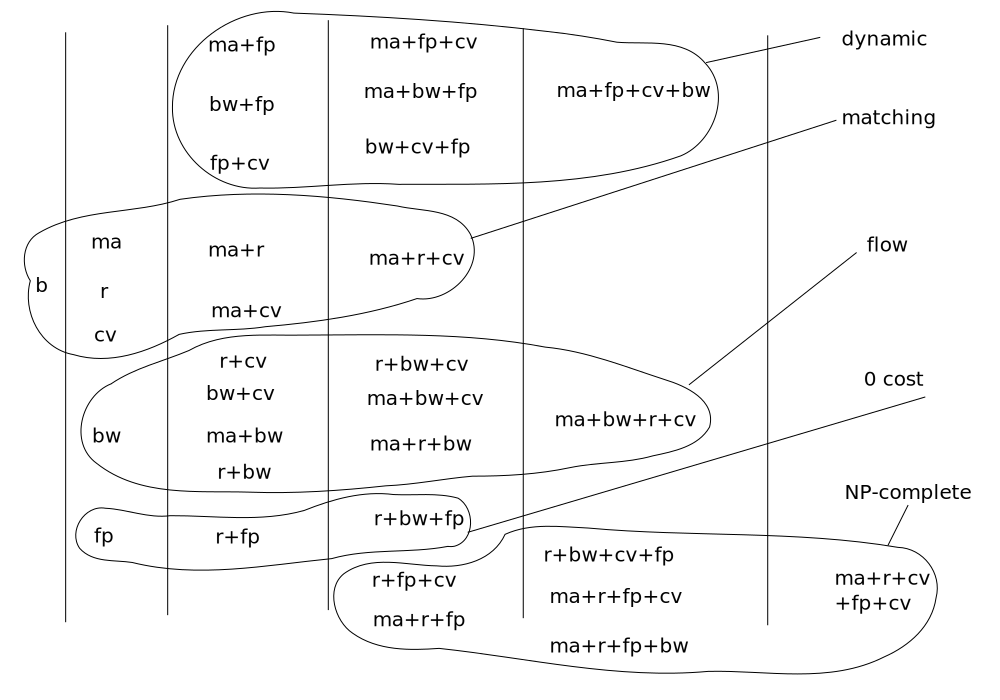
\includegraphics[width = \columnwidth]{figs/summary}
\caption{foo}
\label{fig:summary}
\end{figure}



%%%%%%%%%%%%%%%%%%%%%%%%%%%%%%%%%%%%%
\subsection{Dynamic programming solution to single virtual cluster
  embedding, footprint minimization, one chunk per VM}
Model:
\begin{itemize}
  \item We are given a tree $T$ with capacities $c_e$ on the edges
    (physical network)easured in number of edges)
  \item We are given $n$ chunks that are assigned to leaves of $T$ (at
    most one chunk to one leaf)
  \item Our task is to place $n$ virtual machines on leaves of $T$ (at
    most one virtual machine to one leaf)
  \item Virtual machines can be placed directly on empty leaves or on leaves with chunks
  \item Each chunk has to be transferred to a virtual machine (matching), and the
    cost inlined by that is equal to $b_1$ times distance between
    chunk and virtual machine measured by number of edges
  \item Each virtual machine has to communicate with each other
    virtual machine, and the cost inclined by that is equal to $b_2$
    times distance between each pair of virtual machines meas total cost
\end{itemize}

Let's start by transforming our tree to binary tree with arbitrary
depth. We also introduce weights on edges (either $0$ or $1$). The
strategy we use is to clone every vertex $|children(v)| - 2$ times,
placing subsequent clones as right son of the previous one and placing
subsequent children as left son of the clone. Last child is placed as
right son of last clone.

Let's begin designing our algorithm by writing recursive formula for
minimal cost inclined by placing virtual machines in leaves of a given
tree. Our approach is to evaluate this function using bottom-up
technique using auxilary array, which yields a dynamic programming
solution. To find actual placements of virtual machines in addition to
the cost, we traverse the array backwards, following the path of
minimas.

Keep in mind that number of virtual machines is equal to number of
chunks. However, our function $f$ will be defined by structural
induction on the tree and we will invalidate the property of having
the same number of chunks and virtual machines in a given subtree (which is true when
we look at whole tree).

Let's define $f$ in following way. First argument is a subtree (with
available informations like number of chunks in its leaves), and the
second argument is number of virtual machines that we decided to place
in the subtree (given as first parameter). To calculate optimum
placement of $x$ virtual machines in subtree $T$ ($f(T, x)$) we will
consider every possible split of number $x$ into two positive integer
values: $l$ and $r = x - l$. We will place $l$ virtual machines in
left subtree of $T$ and $r$ virtual machines in right subtree of
$T$. Having such information allow us to compute how much cost we
incline through edge $e_1$ (which connects left subtree of $T$ to root
of $T$) and edge $e_2$ (which connects right subtree of $T$ to root of
$T$). In a given recursive call we charge only those two edges, rest
of edges will be charged is subsequent calls.

Our cost function consists of two factors. First one, communication cost
between virtual machines is easy to compute. We know how many virtual
machines are in left subtree, how many are in right subtree and how
many are in whole tree outside of $T$. For each pair of virtual
machines, first of which is in left subtree and second of which is in
right subtree, we charge $b_2 \cdot (w(e_1) + w(e_2))$. For each pair
of virtual machines, first of which is in left subtree and second of
which is outside $T$, we charge $b_2 \cdot w(e_1)$. Right subtree case
is symmetrical. Second factor of our cost function is the cost of
transferring chunks to virtual machines. Let's call number of chunks
in left subtree as $c_l$ and number of chunks in right subtree as
$c_r$. To incline minimal cost we connect chunks in given subtree to
virtual machines in the same subtree. If we can no longer do that,
because $v_i < c_i (i \in \{l,r\})$, then we connect leftover chunks
to virtual machines in second subtree of $T$. If we can no longer do
that, we connect leftover chunks outside of $T$. This strategy is
optimal, because connecting any other way can be amended (TODO: need
better argument here), inclining lower cost. Connections inside either
left or right subtrees inclines cost $0$ to edges $e_1$ and
$e_2$. Connections between left and right subtree incline cost $b_1
\cdot (w(e_1) + w(e_2))$. Connections from either subtree to outside
of $T$ inclines either $b_1 \cdot w(e_1)$ or $b_2 \cdot
w(e_2)$. Finally, we can write down our formula for $f$:

$$ f(T, x) = min_{l \in \{0, \ldots, x\}} \{ f(T_l, l) + f(T_r, x - l)
+ TransferCost + ConnectionCost\} $$

where $TransferCost$ and $ConnectionCost$ are constants independent of
$l$, and are defined in paragraph above. One simplifying observation
is that to calculate $ConnectionCost$ we can just use the absolute
value of difference
between number of chunks and number of virtual machines in a given
subtree, without knowing which is bigger, because in our model if
there are some virtual machines left, we know that some chunks from
outside will use the same transfer as if we have excessive chunks in
the subtree.

Regarding base case we
trivially define leaf case as having cost $0$ if $x = 0$, cost $b_2
\cdot (n-1) + b_1\cdot n$ if there is no chunk in the leaf, cost $b_2 \cdot (n-1) +
b_1 \cdot (n-1)$ if there is a chunk in the leaf and $\infty$ otherwise.

Capacity constraints are preserved in such way that we put $f(T, x) =
\infty$ if either $e_1$ or $e_2$ transfer cost added to communication
cost exceedes its capacity. Doing so guarantees that this
(impossible) case can never be chosen as a minimum on higher levels of
recurrence calls (unless all other ways are impossible as well). 

When it comes to time complexity of described algorithm, we spend
certain amount of time in every of $2|T|$ vertices of binary
tree (2 is there because of binary transformation). This time can be
bound by iterating over splits of $n$ into two integers, times some
constant and we do it for every possible number of VMs from $0$ to $n$. Therefore, resulting running time is $O(Nn^2)$.


%%%%%%%%%%%%%%%%%%%%%%%%%%%%%%%%%%%%%%
\subsection{Dynamic programming solution to single virtual cluster
  embedding, footprint minimization, VMs have unlimited processing power}
Model will be a modification of model from previous chapter. The only
difference is that each VM can process arbitrary amount of chunks
instead of only one.

Our approach will be tree binarization, followed by dynamic
programming algorithm. This time, instead of just having one array
with costs, now we have 3 arrays, named cost[T, x], up[T, x] and
down[T, x]. Array cost[T, x] is the
same as previously, the sum of bandwidth allocated in subtree T,
knowing that it contains x VMs. Array up[T, x] is amount of transfer
from chunks that did not fit inside tree T because of capacity
constraints and have to be pointed outside. Array down[T, x] is amount
of processing power of the subtree; in other words it is the amount of
transfer that can be pointed towards VMs in T. Both up[T,x] and
down[T,x] are closely related to cost[T,x] in the sense that we assume
that the same decisions about placing VMs were taken in up, down as in
cost.



%%%%%%%%%%%%%%%%%%%%%%%%%%%%%%%%%%%%%
\section{Appendix}

%%%%%%%%%%%%%%%%%%%%%%%%%%%%%%%%%%%%%
\bibliographystyle{alpha}
\bibliography{references}

\end{document}
